\documentclass[a4paper,11pt]{scrartcl}

\usepackage[utf8]{inputenc}
\usepackage[ngerman]{babel}

\usepackage{amsmath}
\usepackage{amsfonts}
\usepackage{amssymb}

\usepackage{listings}

\usepackage{enumerate}
\usepackage{xspace}

\usepackage[pdftex]{graphicx}
\usepackage[update]{epstopdf}
\usepackage{hyperref,breakurl}

\renewcommand{\vec}[1]{\mathbf{#1}}
\newcommand{\vr}{\vec{r}}
\newcommand{\vp}{\vec{p}}
\newcommand{\E}{\mathbf{e}}
\newcommand{\I}{\mathrm{i}}
\newcommand{\ind}[1]{_\mathrm{#1}}

\newcommand*{\ov}[2]{{{\vphantom{I}}^{#1}{\vphantom{I}}_{#2}}}
\newcommand*{\uv}[2]{{{\vphantom{I}}_{#1}{\vphantom{I}}^{#2}}}
\newcommand*{\Sr}[2][0]{\rule[#1ex]{0pt}{#2ex}}
\newcommand*{\zB}{z.\,B.\xspace }
\newcommand*{\dH}{d.\,h.\xspace }
\newcommand*{\iA}{i.\,a.\xspace }
\newcommand*{\uA}{u.\,a.\xspace}
\newcommand*{\vH}{\,\%\xspace}
\newcommand*{\dD}{\ensuremath{\mkern1mu\mathrm{d}}}
\newcommand*{\diff}[3][]{\frac{\dD^{#1}{#2}}{\dD^{}{#3}{}^{#1}}}
\newcommand*{\pdiff}[3][]{\frac{\partial^{#1}{#2}}{\partial^{}{#3}{}^{#1}}}
\newcommand*{\ArrF}[1]{\renewcommand{\arraystretch}{#1}}
\newcommand*{\Z}[1]{\ensuremath{\cdot10^{#1}}}
\newcommand*{\G}{\ensuremath{{}^{\circ}}\xspace}
\newcommand*{\GC}{\,\ensuremath{{}^{\circ}\text{C}}\xspace}
\newcommand*{\GF}{\,\ensuremath{{}^{\circ}\text{F}}\xspace}\let\sG\G % wg circ
\newcommand*{\entspricht}{\stackrel{\scriptscriptstyle\wedge}{=}}

\newcommand*{\nfrac}[2]{\nicefrac{#1}{#2}}

\renewcommand*{\bar}[1]{\overline{#1}}

\newcommand{\qed}{\hfill\ensuremath{\Box}}

\parindent0pt

% Title Page
% \title{Statistische Physik II - 3. Übungsblatt}
% \author{Dortje Schirok\\Christoph Tavan\\Patric Zimmermann}
% \date{9. Mai 2011}
\pagestyle{empty}

\begin{document}

\section*{Aufgabe 15 und 17} % (fold)
\label{sec:aufgabe_15}
Wir betrachten einen Massepunkt im Zentralpotential \begin{align}
	\Phi(r) = - \frac{1}{r} \quad\text{mit}\quad r = \sqrt{x^2+y^2} .
\end{align}
Auf das Teilchen wirkt also eine Kraft \begin{align}
	\vec{F}(\vec{r}) = -\nabla \Phi(r) = - \frac{\vec{r}}{r^3} = - \frac{1}{(x^2+y^2)^{3/2}} \left(
	\begin{array}{c}
	x
	\\ y\end{array} \right) .
\end{align}
Eine Kreisbahn (als Beispiel für eine geschlossene Bahn) erhält man wenn diese Kraft gerade die Zentripetalkraft kompensiert: \begin{align}
	\frac{m v^2}{r} \vec{e}_r &= \frac{r}{r^3} \vec{e}_r\\
	\Rightarrow\quad v &= \pm \frac{1}{\sqrt{m r}} 
\end{align}
Anfangsbedingungen, für die diese Bedingung erfüllt ist, sind also \zB \begin{align}
	\vec{r}(t=0) &= \left(
	\begin{array}{c}
	r_0\\ 
	0\end{array} \right)\\
	\vec{v}(t=0) &= \left(
	\begin{array}{c}
	0\\ 
	v_0 \end{array} \right) \quad\text{mit}\quad v_0 = (m r_0)^{-1/2}.
\end{align}
Der Verlet-Algorithmus benötigt den Ort $\vec{r}(t=0)$ sowie den Ort im darauffolgenden Zeitschritt $\vec{r}(t=0+\delta t)$ als Anfangsbedingungen, wobei der zweite Ort anhand der Anfangsgeschwindigkeit ermittelt werden muss. Da wir eine Kreisbewegung fordern, fordern wir, dass der Abstand zum Ursprung erhalten bleibt. Für den Ort nach einem Zeitschritt ergibt sich dann näherungsweise \begin{align}
	\vec{r}(t=0+\delta t) &= \left(
	\begin{array}{c}
	\sqrt{r_0^2 - (v_0\,\delta t)^2 } \\ 
	v_0\,\delta t \end{array} \right).
\end{align}
In der Praxis muss der Zeitschritt $\delta t$ dann klein genug gewählt werden, damit diese Näherung wirklich auf kreisförmige Bahnen führt. In unserer Simulation musste für eine Bahn mit Radius 1 für den Verlet-Algorithmus $\delta t \sim 0.001$ gewählt werden.

\subsubsection*{Vergleich Verlet $\leftrightarrow$ Leap Frog} % (fold)
\label{ssub:vergleich_verlet_leftrightarrow_leap_frog}
Wie man aus den Plots der Trajektorien in Abb. \ref{fig:traj} erkennen kann, liefert der Verlet-Algorithmus bei gleichem Zeitschritt geringere Abweichungen von der theoretisch zu erwartenden Kreisbahn. Auch bei der Entwicklung der Energien, die in Abb. \ref{fig:en} dargestellt sind, liefert der Verlet-Algorithmus eine bessere Stabilität.

\begin{figure}[tbp]
\centering
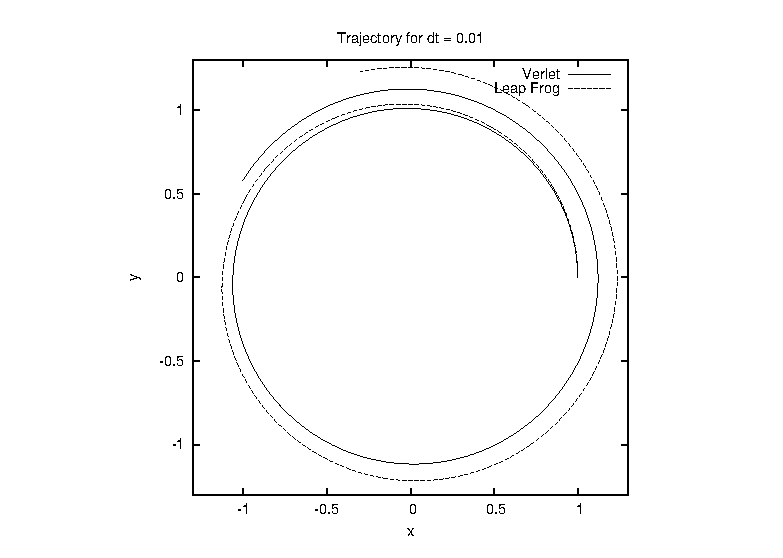
\includegraphics[width=0.8\textwidth]{../trajectories_0_01}\\ 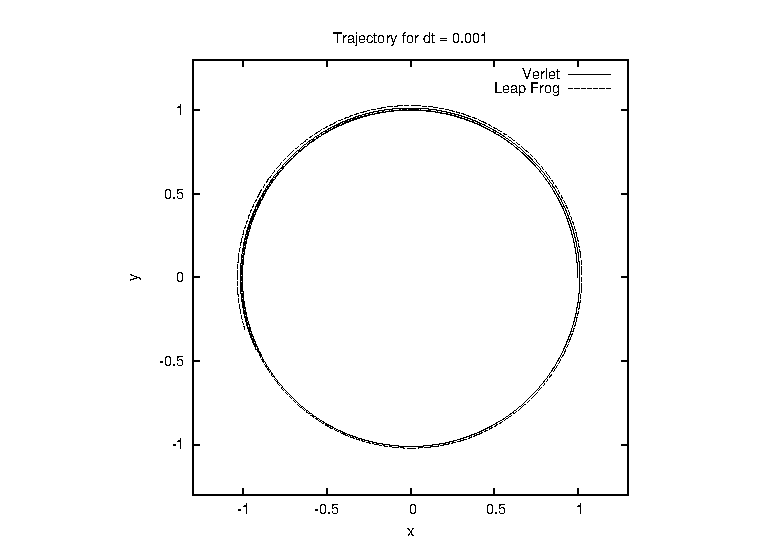
\includegraphics[width=0.8\textwidth]{../trajectories_0_001}\\
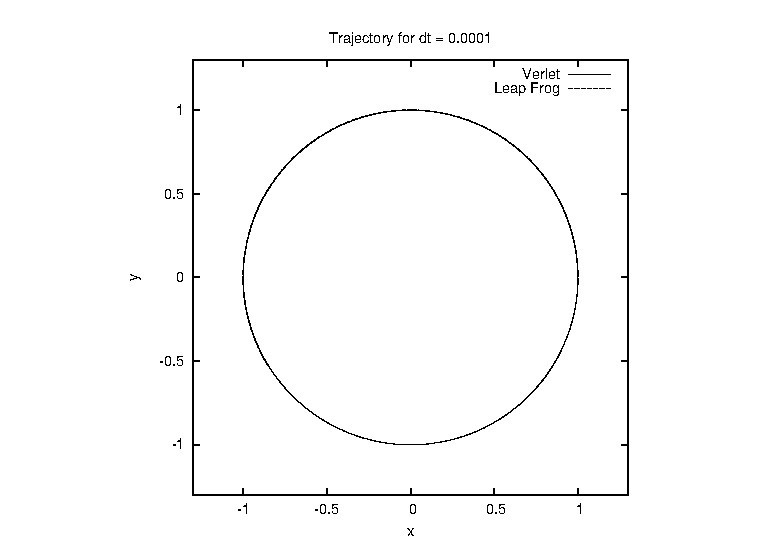
\includegraphics[width=0.8\textwidth]{../trajectories_0_0001}
\caption{Trajektorien für verschieden lange Zeitschritte.}\label{fig:traj}
\end{figure}


\begin{figure}[tbp]
\centering
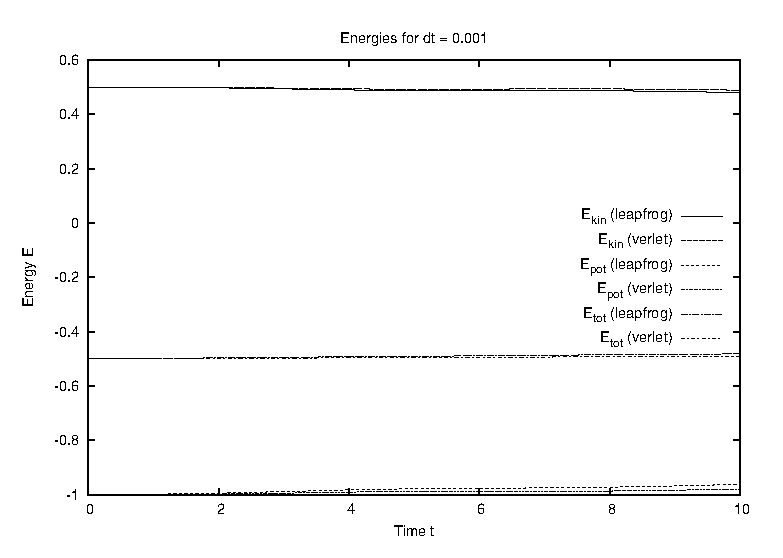
\includegraphics[width=1.0\textwidth]{../energies_0_001}
\caption{Zeitliche Entwicklung von kinetischer, potentieller und Gesamt-Energie.}\label{fig:en}
\end{figure}

% subsubsection vergleich_verlet_leftrightarrow_leap_frog (end)
% section aufgabe_15 (end)

\subsubsection*{Virial-Theorem} % (fold)
\label{ssub:virial_theorem}
Das Virialtheorem \begin{align}
	\left\langle E_{pot} \right\rangle  = - 2 \left\langle E_{kin} \right\rangle 
\end{align}
konnte ebenfalls bestätigt werden. Im folgenden ist die Ausgabe des Programms nach 1000 Zeitschritten der Länge $\delta t = 0.01$ aufgeführt. Dabei wurde die Abweichung des Wertes $\left\langle E_{pot} \right\rangle  + 2 \left\langle E_{kin} \right\rangle$ von Null berechnet. Mit dem Leap Frog Algorithmus ergibt sich:
\begin{lstlisting}
Averages:
Kinetic energy:		0.434153
Potential energy:	-0.865105
Total energy:		-0.430951
Virial theorem <E_pot> = - 2 <E_kin>.
  Difference:		0.00320218
  Relative Diff.:	0.004 %
\end{lstlisting}
Und mit dem Verlet Algorithmus:
\begin{lstlisting}
Averages:
Kinetic energy:		0.463277
Potential energy:	-0.922384
Total energy:		-0.459107
Virial theorem <E_pot> = - 2 <E_kin>.
  Difference:		0.00417052
  Relative Diff.:	0.005 %
\end{lstlisting}
Die Übereinstimmung wird immer besser, je mehr Zeitschritte ausgeführt werden.
% subsubsection virial_theorem (end)

\end{document}

